\chapter{Rotation Invariant Local Binary Convolution Neural Networks}

{\small \textbf{Authors}\\
XIN ZHANG, YUXIANG XIE, JIE CHEN, (Member, IEEE), LINGDA WU, QIXIANG YE, (Senior Member, IEEE), AND LI LIU\\ \\
IEEE Access\\VOLUME 6, 2018}

\section{Proposed Method}
 
Despite what it has been seen in the previous paper, the problem of the feature invariance is covered also here but with a very different approach. In fact, previously it has been dealt more with distances in manifolds representing classes. On the other hand, in this paper, a new architecture for CNNs is proposed, whose aim is to increase the ability of our network to handle features invariance. The problem itself is how to deal with objects that might change in position and more. It is worth pointing out that some of the advice given in this paper are in disagreement with the previous one. For example, data augmentation has been slightly criticized before, because it does not improve more than 1\% performance if we increase training samples from 1M to 14M. On the other hand, in the following work it is highly recommended. Moreover, data augmentation can be pursued through two different approaches. The first one seems to be the handcrafted design of the features we are looking for but it is such a heavy and slow process and is not that efficient. Otherwise, there is the classical approach to perform basic operations to enlarge our dataset, where we end up with a higher invariance. As this is only a precondition, let us see now what is the proposed method about. A new CNN is proposed and it is called \textit{Rotation Invariant Local Binary Convolutional Neural Network} (RI-LBCNN) that basically is a new architecture in which a module is added. This module is the \textit{Local Binary orientation Module} (LBoM). The main difference between a common CNN and a LBCNN is that the convolutional layer is replaced with something called Local Binary Convolution (LBConv) that is able to achieve the same performance of CNNs but with fewer parameters. The following module is made of three layers. The first two make up the first component, while the other layer makes up the second one. More specifically, what is done in this module is to use binary filters that we initialize through a Bernoulli distribution. At the same time, while we are performing the convolution operation, we properly rotate these filters in order to obtain other orientation channels. An illustration of the whole module architecture is shown in Figure \ref{fig:05_1}. As we can see, in the first component, there are the two mentioned layers where through activations we end up with bit maps, then we move to the second component where features maps are obtained as output.\\

\begin{figure}[h!]
    \centering
    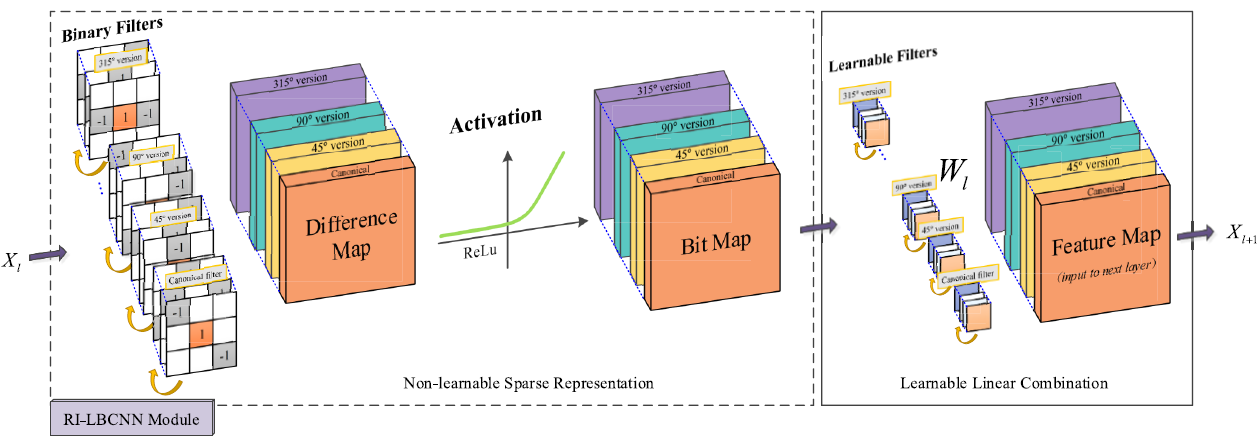
\includegraphics[scale=0.45]{images/05_1.png}
    \caption{Local Binary orientation Module (LBoM) in RI-LBCNNs.}
    \label{fig:05_1}
\end{figure}

\FloatBarrier
 
\section{Experimental Results}

Let us now move into experimental results. The datasets used here are the MNIST \citep{MNIST} and other two its variants that are MNIST-rot-12k and MNIST-rot. These two variants are still based on the original MNIST but they are built in order to better face the rotation-variant problem. After having carried out a few tests, some among the most known CNN architectures such as VGGNet, ResNet and WideResNet are used to deal with an image classification problem with other two datasets that are CIFAR10 \citep{CIFAR10and100} and CIFAR100 \citep{CIFAR10and100}. It turns out that CNNs using the proposed LBoM module outperform the aforementioned architectures that do not use it. 
